

\usepackage{tikz}
\usetikzlibrary{arrows.meta,positioning,calc,fit,decorations.pathreplacing,shapes}


% ---------------------------------------------------
% Slide: SimpleBackbone diagram (YOLO demo)
% Requires in preamble:
% \usepackage{tikz}
% \usetikzlibrary{arrows.meta,positioning,fit,calc,shapes}
% ---------------------------------------------------
\begin{frame}[fragile]{SimpleBackbone (Tiny CNN)}
    \centering
    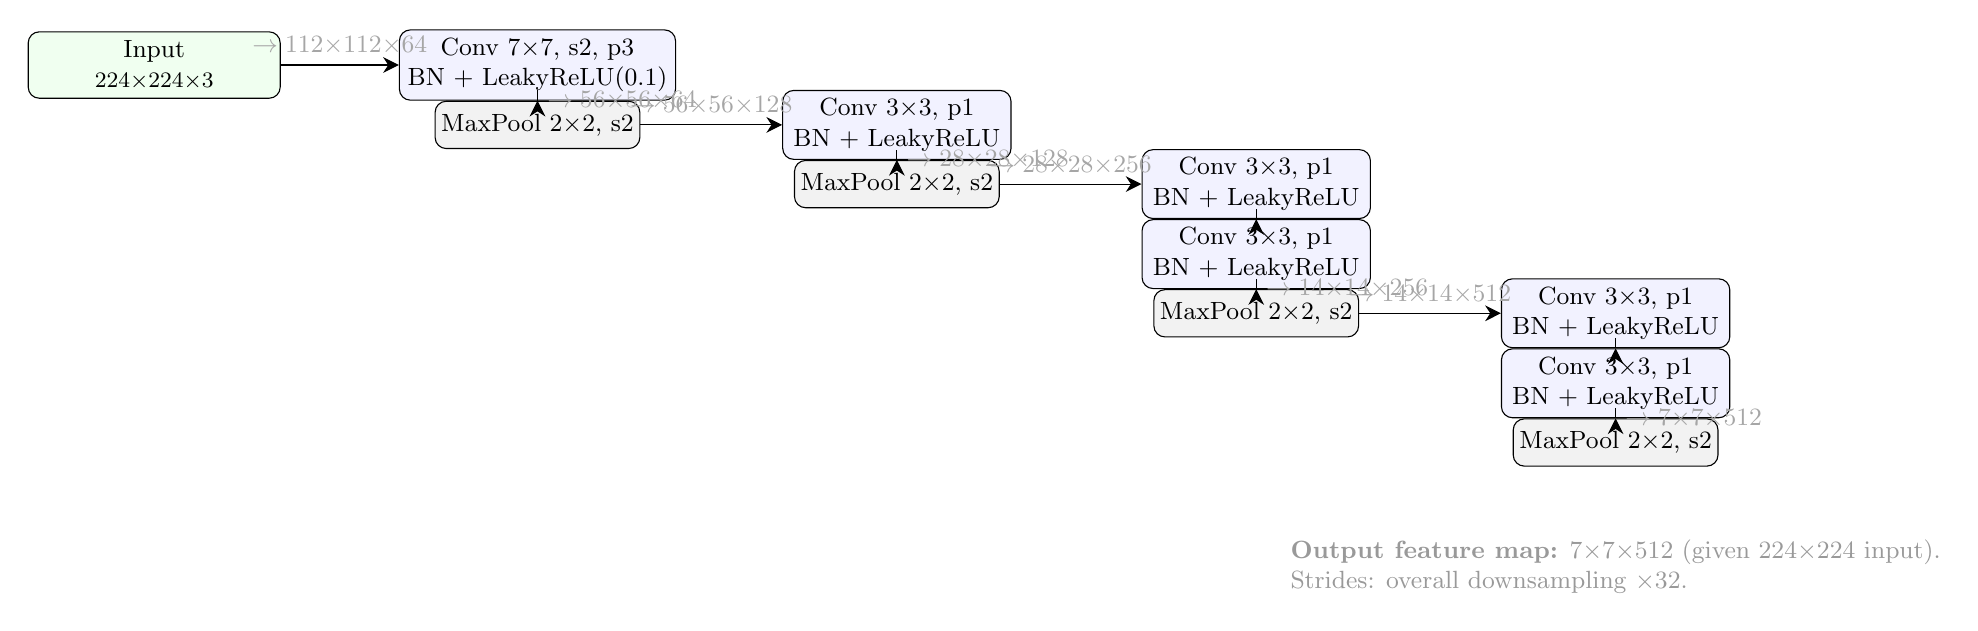
\begin{tikzpicture}[
      font=\small,
      node distance=8mm and 8mm,
      box/.style={draw, rounded corners, align=center, inner sep=3pt, minimum width=2.9cm, minimum height=8mm, fill=blue!5},
      op/.style={draw, rounded corners, align=center, inner sep=2pt, minimum width=2.6cm, minimum height=6mm, fill=gray!10},
      every edge quotes/.style={auto, text=gray!70},
      >={Stealth[length=2mm,width=2mm]}
    ]
    % Input
    \node[box, fill=green!6, minimum width=3.2cm] (in) {Input\\\footnotesize $224{\times}224{\times}3$};
    
    % Block 1
    \node[box, right=15mm of in] (c1) {Conv $7{\times}7$, s2, p3\\ BN + LeakyReLU(0.1)};
    \node[op, below=0mm of c1] (p1) {MaxPool $2{\times}2$, s2};
    \draw[->] (in) -- (c1) node[midway, above, text=gray!70] {$\to 112{\times}112{\times}64$};
    \draw[->] (c1) -- (p1) node[midway, right, text=gray!70] {$\to 56{\times}56{\times}64$};
    
    % Block 2
    \node[box, right=18mm of p1] (c2) {Conv $3{\times}3$, p1\\ BN + LeakyReLU};
    \node[op, below=0mm of c2] (p2) {MaxPool $2{\times}2$, s2};
    \draw[->] (p1) -- (c2) node[midway, above, text=gray!70] {$\to 56{\times}56{\times}128$};
    \draw[->] (c2) -- (p2) node[midway, right, text=gray!70] {$\to 28{\times}28{\times}128$};
    
    % Block 3 (two convs)
    \node[box, right=18mm of p2] (c3a) {Conv $3{\times}3$, p1\\ BN + LeakyReLU};
    \node[box, below=0mm of c3a] (c3b) {Conv $3{\times}3$, p1\\ BN + LeakyReLU};
    \node[op,  below=0mm of c3b] (p3) {MaxPool $2{\times}2$, s2};
    \draw[->] (p2) -- (c3a) node[midway, above, text=gray!70] {$\to 28{\times}28{\times}256$};
    \draw[->] (c3a) -- (c3b);
    \draw[->] (c3b) -- (p3) node[midway, right, text=gray!70] {$\to 14{\times}14{\times}256$};
    
    % Block 4 (two convs)
    \node[box, right=18mm of p3] (c4a) {Conv $3{\times}3$, p1\\ BN + LeakyReLU};
    \node[box, below=0mm of c4a] (c4b) {Conv $3{\times}3$, p1\\ BN + LeakyReLU};
    \node[op,  below=0mm of c4b] (p4) {MaxPool $2{\times}2$, s2};
    \draw[->] (p3) -- (c4a) node[midway, above, text=gray!70] {$\to 14{\times}14{\times}512$};
    \draw[->] (c4a) -- (c4b);
    \draw[->] (c4b) -- (p4) node[midway, right, text=gray!70] {$\to 7{\times}7{\times}512$};
    
    % Output note
    \node[align=left, text=gray!80, below=8mm of p4] (note) {%
    \textbf{Output feature map:} $7{\times}7{\times}512$ (given $224{\times}224$ input).\\
    Strides: overall downsampling $\times 32$.%
    };
    
    \end{tikzpicture}
    \end{frame}
    


% ---------------------------------------------------
% Slide: YOLODetector block/data flow
% Requires in preamble:
% \usepackage{tikz}
% \usetikzlibrary{arrows.meta,positioning,fit,calc,shapes,backgrounds}
% ---------------------------------------------------
\begin{frame}[fragile]{YOLODetector: End-to-End Data Flow}
    \centering
    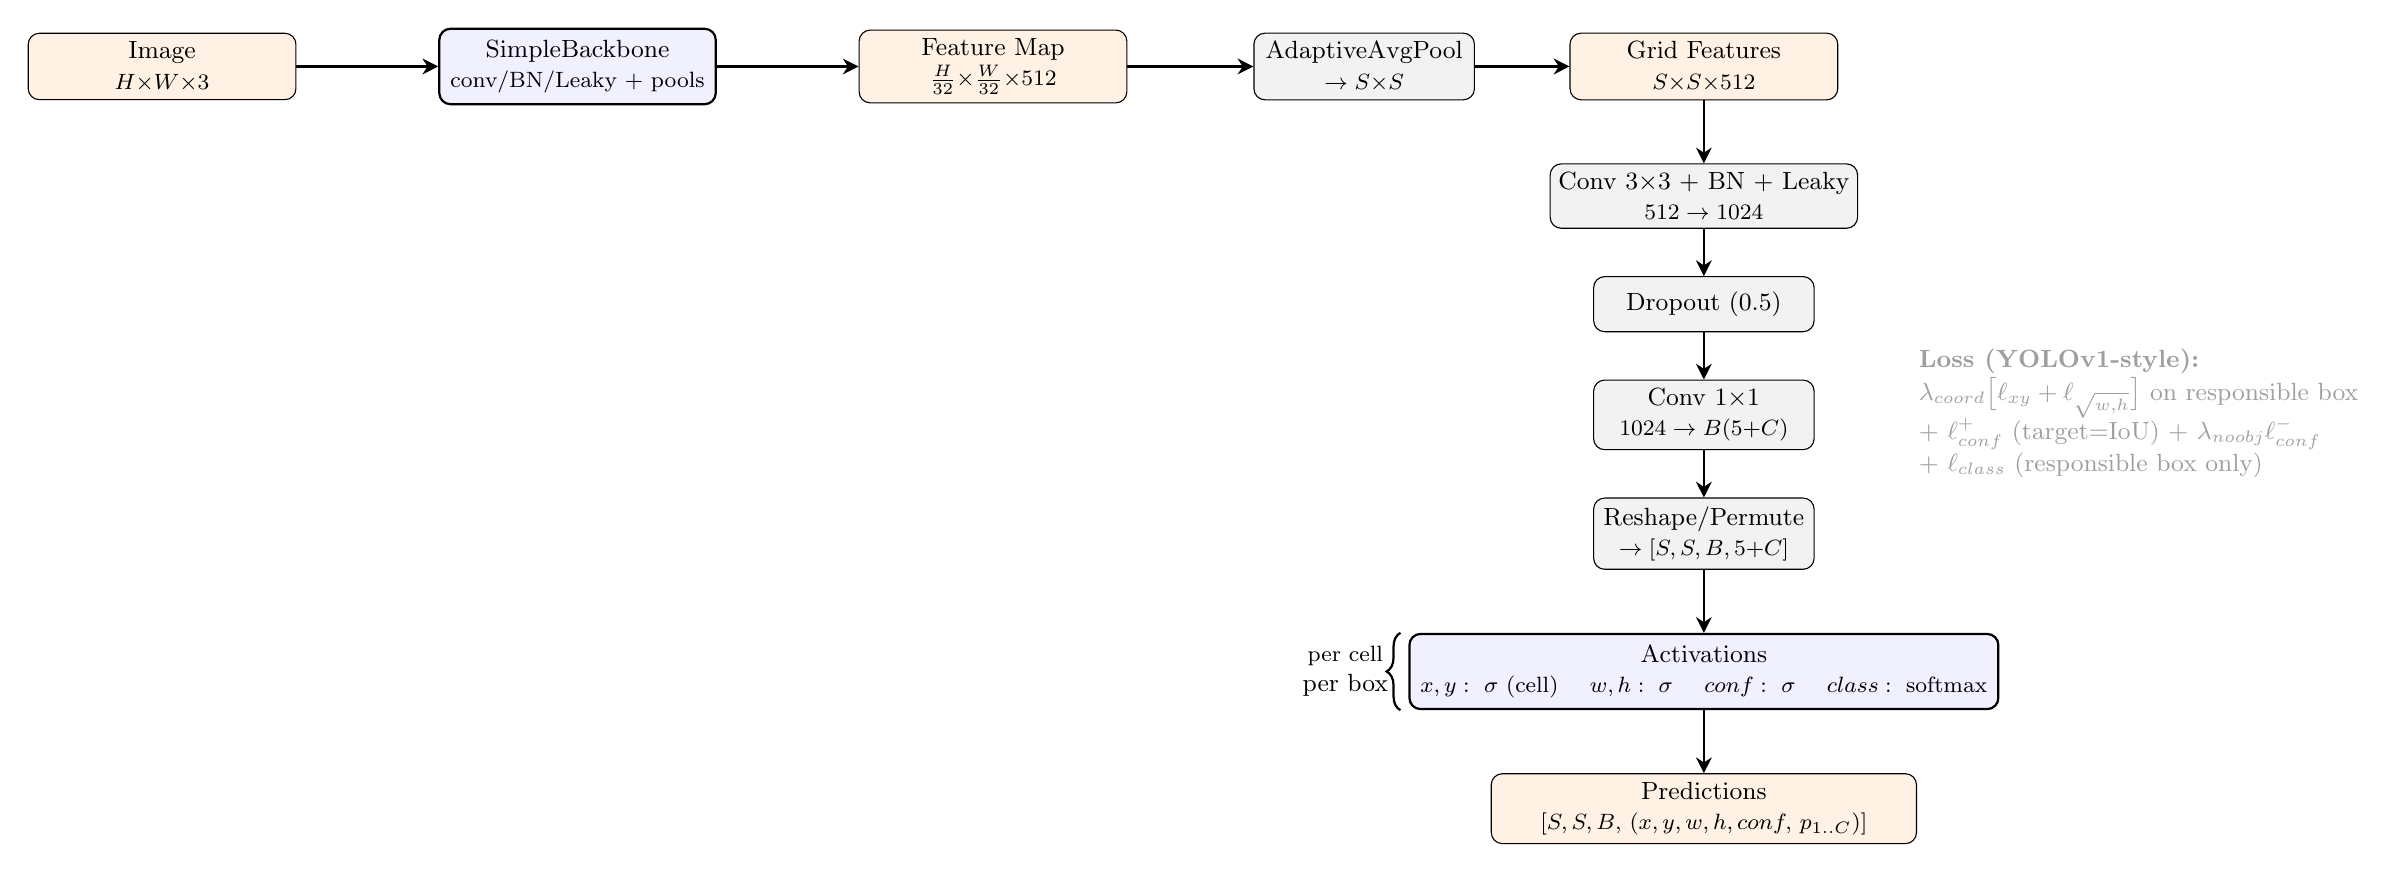
\begin{tikzpicture}[
      font=\small,
      node distance=10mm and 10mm,
      stage/.style={draw, rounded corners, thick, fill=blue!6, inner sep=4pt, align=center, minimum width=3.2cm, minimum height=9mm},
      op/.style={draw, rounded corners, fill=gray!10, inner sep=3pt, align=center, minimum width=2.8cm, minimum height=7mm},
      tensor/.style={draw, rounded corners, fill=orange!10, inner sep=3pt, align=center, minimum width=3.4cm, minimum height=7mm},
      >={Stealth[length=2mm,width=2mm]}
    ]
    
    % Input
    \node[tensor] (img) {Image\\\footnotesize $H{\times}W{\times}3$};
    
    % Backbone
    \node[stage, right=18mm of img] (bb) {SimpleBackbone\\\footnotesize conv/BN/Leaky + pools};
    \draw[->, thick] (img) -- (bb);
    
    % Backbone output
    \node[tensor, right=18mm of bb] (feat) {Feature Map\\\footnotesize $\frac{H}{32}{\times}\frac{W}{32}{\times}512$};
    \draw[->, thick] (bb) -- (feat);
    
    % Adaptive Pool to SxS
    \node[op, right=16mm of feat] (pool) {AdaptiveAvgPool\\\footnotesize $\to S{\times}S$};
    \draw[->, thick] (feat) -- (pool);
    
    \node[tensor, right=12mm of pool] (grid) {Grid Features\\\footnotesize $S{\times}S{\times}512$};
    \draw[->, thick] (pool) -- (grid);
    
    % Detection head 3x3
    \node[op, below=8mm of grid] (head1) {Conv $3{\times}3$ + BN + Leaky\\\footnotesize $512 \to 1024$};
    \draw[->, thick] (grid) -- (head1);
    
    % Dropout (optional)
    \node[op, below=6mm of head1] (drop) {Dropout (0.5)};
    \draw[->, thick] (head1) -- (drop);
    
    % 1x1 conv to output channels
    \node[op, below=6mm of drop] (head2) {Conv $1{\times}1$\\\footnotesize $1024 \to B(5{+}C)$};
    \draw[->, thick] (drop) -- (head2);
    
    % Reshape
    \node[op, below=6mm of head2] (reshape) {Reshape/Permute\\\footnotesize $\to [S,S,B,5{+}C]$};
    \draw[->, thick] (head2) -- (reshape);
    
    % Activations
    \node[stage, below=8mm of reshape, minimum width=5.2cm] (acts) {Activations\\
    \footnotesize $x,y:\ \sigma$ (cell) \quad $w,h:\ \sigma$ \quad $conf:\ \sigma$ \quad $class:\ \mathrm{softmax}$};
    \draw[->, thick] (reshape) -- (acts);
    
    % Predictions
    \node[tensor, below=8mm of acts, minimum width=5.4cm] (pred) {Predictions\\\footnotesize $[S,S,B,\, (x,y,w,h,conf,\,p_{1..C})]$};
    \draw[->, thick] (acts) -- (pred);
    
    % Side notes
    \node[align=left, text=gray!75, right=12mm of head2] (note) {%
    \textbf{Loss (YOLOv1-style):}\\
    \begin{tabular}{@{}l@{}}
    $\lambda_{\text{coord}}\big[\ell_{xy}+\ell_{\sqrt{w,h}}\big]$ on responsible box\\
    $+\ \ell_{\text{conf}}^{+}$ (target=IoU) $+\ \lambda_{\text{noobj}}\ell_{\text{conf}}^{-}$\\
    $+\ \ell_{\text{class}}$ (responsible box only)
    \end{tabular}};
    
    % Braces for shapes
    \draw[decorate, decoration={brace, amplitude=5pt}, thick]
      ($(acts.south west)+(-0.1,0)$) -- ($(acts.north west)+(-0.1,0)$)
      node[midway, xshift=-7mm, align=center] {\footnotesize per cell\\per box};
    
    \end{tikzpicture}
    \end{frame}
    



    % ---------------------------------------------------
% Slide: Cell-relative to Absolute Coordinates (YOLO grid)
% ---------------------------------------------------
\begin{frame}[fragile]{From Cell-Relative to Absolute Coordinates}
    \begin{columns}[T,onlytextwidth]
    \begin{column}{0.55\textwidth}
    \centering
    \begin{tikzpicture}[
      font=\small,
      >={Stealth[length=2mm,width=2mm]},
      cell/.style={draw,minimum width=1.1cm,minimum height=1.1cm},
      gridlab/.style={text=gray!60},
      hl/.style={draw=blue!70,very thick,fill=blue!5},
      ctr/.style={circle, draw=blue!80, fill=blue!20, inner sep=1.2pt},
      vec/.style={->,thick,blue!80}
    ]
    % Parameters
    \def\S{7}
    \def\ii{3} % i (row)
    \def\jj{4} % j (col)
    
    % Grid SxS
    \foreach \y in {0,...,6}{
      \foreach \x in {0,...,6}{
        \node[cell] (c-\x-\y) at (\x*1.1, -\y*1.1) {};
      }
    }
    % Highlight cell (i,j)
    \node[hl, fit=(c-\jj-\ii)] (hcell) {};
    
    % Axes / labels
    \node[gridlab, above=1mm of c-0-0.north west, anchor=south west] {$S{\times}S$ grid};
    \node[gridlab, above=0mm of c-\jj-\ii.north] {$(i{=}\ii,\ j{=}\jj)$};
    
    % Cell-local origin and predicted center
    \coordinate (cellNW) at (c-\jj-\ii.north west);
    \coordinate (cellSE) at (c-\jj-\ii.south east);
    \path (cellNW) -- (cellSE) coordinate[pos=0.5] (cellC);
    
    % Local axes
    \draw[gray!50,->] (cellNW) ++(0.05,-0.05) -- ++(0.85,0) node[midway, above, gridlab] {$x_{\text{cell}}\in(0,1)$};
    \draw[gray!50,->] (cellNW) ++(0.05,-0.05) -- ++(0,-0.85) node[midway, left, gridlab] {$y_{\text{cell}}\in(0,1)$};
    
    % Example offsets in the highlighted cell
    \coordinate (localO) at ($(cellNW)+(0.05,-0.05)$);
    \def\xcell{0.6}
    \def\ycell{0.35}
    \coordinate (predC) at ($(localO)+(\xcell*0.85,-\ycell*0.85)$);
    \node[ctr,label={[blue!80]above:Pred center $(x_{\text{cell}},y_{\text{cell}})$}] (pC) at (predC) {};
    
    % Absolute center arrow (to global normalized coords)
    % Global normalized axes (0..1) across full image
    \draw[gray!60, ->] (-0.8,0.5) -- (8.0,0.5) node[right, gridlab] {$x \in [0,1]$};
    \draw[gray!60, ->] (-0.8,0.5) -- (-0.8,-8.2) node[below, gridlab] {$y \in [0,1]$};
    
    % Convert to absolute center: (j + x_cell)/S, (i + y_cell)/S
    \coordinate (absC) at ($(-0.8,0.5) + ((\jj+\xcell)/\S*8.8, -(\ii+\ycell)/\S*8.7)$);
    \draw[vec] (pC) to[bend right] node[midway, right, xshift=1mm] {\footnotesize abs. center} (absC);
    \node[ctr, fill=orange!30, draw=orange!80, label={[orange!80]right:$(x,y)$}] at (absC) {};
    
    % Width/height visualization (relative to image)
    \def\ww{0.22}  % example w
    \def\hh{0.14}  % example h
    \draw[orange!80, thick] ($(absC)+(-\ww*4.4, \hh*4.35)$) rectangle ($(absC)+(\ww*4.4, -\hh*4.35)$);
    
    % Cell index braces
    \draw[decorate, decoration={brace, amplitude=4pt}, gray!60]
      ($(c-\jj-0.north)+(-0.55,0.1)$) -- ($(c-\jj-6.south)+(-0.55,-0.1)$)
      node[midway, left, gridlab] {$i \in \{0,\dots,S{-}1\}$};
    \draw[decorate, decoration={brace, amplitude=4pt}, gray!60]
      ($(c-0-\ii.west)+(-0.1,0.55)$) -- ($(c-6-\ii.east)+(0.1,0.55)$)
      node[midway, above, gridlab] {$j \in \{0,\dots,S{-}1\}$};
    
    \end{tikzpicture}
    \end{column}
    \begin{column}{0.45\textwidth}
    \small
    \textbf{Predictions per cell, per box ($b$):}
    \[
    (x_{\text{cell}}, y_{\text{cell}}, w, h, \text{conf}, p_{1..C})
    \]
    
    \textbf{Absolute conversion (normalized to $[0,1]$):}
    \[
    x = \frac{j + x_{\text{cell}}}{S},\quad
    y = \frac{i + y_{\text{cell}}}{S}
    \]
    \[
    w_{\text{abs}} = w,\quad
    h_{\text{abs}} = h
    \]
    
    \textbf{Notes:}
    \begin{itemize}
    \item $(i,j)$ are row/col indices of the cell (top-left = $(0,0)$).
    \item $x_{\text{cell}},y_{\text{cell}}\in(0,1)$ are offsets \emph{within} the cell.
    \item $w,h\in(0,1)$ are relative to the whole image.
    \item Pixel coords: multiply by image width/height.
    \end{itemize}
    \end{column}
    \end{columns}
    \end{frame}
    


    % ---------------------------------------------------
% Slide: NMS schematic
% ---------------------------------------------------
\begin{frame}[fragile]{Non-Maximum Suppression (NMS) — Schematic}
    \begin{columns}[T,onlytextwidth]
    \begin{column}{0.55\textwidth}
    \centering
    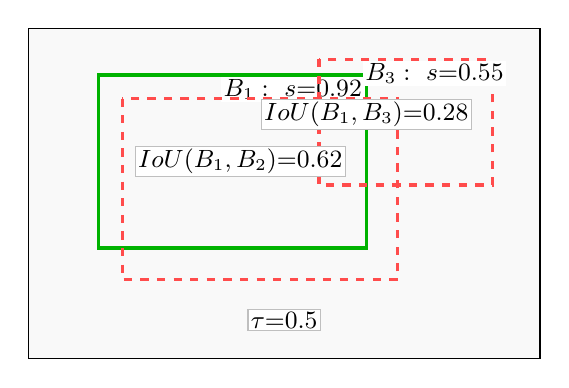
\begin{tikzpicture}[
      font=\small,
      >={Stealth[length=2mm,width=2mm]},
      img/.style={draw, fill=gray!5, minimum width=6.5cm, minimum height=4.2cm},
      keep/.style={draw=green!70!black, very thick},
      suppr/.style={draw=red!70, dashed, very thick},
      lab/.style={fill=white, inner sep=1pt}
    ]
    % Image canvas
    \node[img, anchor=north west] (im) at (0,0) {};
    
    % Three overlapping boxes
    % B1 (highest score) - keep
    \draw[keep] ($(im.north west)+(0.9,-0.6)$) rectangle ++(3.4,-2.2)
      node[lab, anchor=north east] at ($(im.north west)+(4.3,-0.6)$) {$B_1:\ s{=}0.92$};
    
    % B2 - overlaps a lot with B1 -> suppressed
    \draw[suppr] ($(im.north west)+(1.2,-0.9)$) rectangle ++(3.5,-2.3)
      node[lab, anchor=north east] at ($(im.north west)+(4.9,-0.9)$) {$B_2:\ s{=}0.78$};
    
    % B3 - smaller overlap -> may survive
    \draw[suppr] ($(im.north west)+(3.7,-0.4)$) rectangle ++(2.2,-1.6)
      node[lab, anchor=north east] at ($(im.north west)+(6.1,-0.4)$) {$B_3:\ s{=}0.55$};
    
    % IoU annotations
    \node[lab, draw=gray!50] at ($(im.north west)+(2.7,-1.7)$) {$\text{IoU}(B_1,B_2){=}0.62$};
    \node[lab, draw=gray!50] at ($(im.north west)+(4.3,-1.1)$) {$\text{IoU}(B_1,B_3){=}0.28$};
    
    % Threshold
    \node[lab, draw=gray!50] at ($(im.south)+(0,0.5)$) {$\tau{=}0.5$};
    
    \end{tikzpicture}
    \end{column}
    \begin{column}{0.45\textwidth}
    \small
    \textbf{Algorithm (class-wise):}
    \begin{enumerate}
    \item Collect detections $\{(b_k, s_k)\}$ with scores $s_k = \text{conf}\cdot p_{\text{class}}$.
    \item \textbf{Sort} by $s_k$ descending.
    \item Initialize $\mathcal{K} \leftarrow \emptyset$.
    \item While list not empty:
      \begin{enumerate}
      \item Pop highest-score box $b^\*$; add to $\mathcal{K}$.
      \item For each remaining $b$:
        \[
        \text{if } \mathrm{IoU}(b^\*, b) > \tau \text{ then discard } b
        \]
      \end{enumerate}
    \item Return kept set $\mathcal{K}$.
    \end{enumerate}
    
    \textbf{Interpretation here:}
    \begin{itemize}
    \item Keep $B_1$ ($0.92$).
    \item Suppress $B_2$ since $\mathrm{IoU}(B_1,B_2)=0.62>\tau$.
    \item Keep $B_3$ since $0.28<\tau$ (subject to later comparisons).
    \end{itemize}
    
    \textbf{Notes:}
    \begin{itemize}
    \item Run NMS \emph{per class}.
    \item Variants: Soft-NMS (decay scores), DIoU-NMS, class-agnostic NMS, batched NMS.
    \end{itemize}
    \end{column}
    \end{columns}
    \end{frame}
    % ===================================================
% Slide 1 — Why spatial size keeps halving
% ===================================================
\begin{frame}{Backbone Design: Why Do We Keep Halving $H{\times}W$?}
    \textbf{Goal:} grow the \textit{receptive field} (RF) and compress compute/memory.
    
    \medskip
    \textbf{Mechanism:} stride-2 ops halve $H,W$ each stage:
    \[
    224 \;\xrightarrow{\;7\times7,\ s{=}2\;}\; 112
    \;\xrightarrow{\;\text{pool}\;}\; 56
    \;\xrightarrow{\;\text{pool}\;}\; 28
    \;\xrightarrow{\;\text{pool}\;}\; 14
    \;\xrightarrow{\;\text{pool}\;}\; 7
    \quad (\text{overall stride } 32)
    \]
    
    \begin{itemize}
      \item Each downsample $\uparrow$ RF, $\downarrow$ spatial detail.
      \item Efficient: later layers work on smaller maps (cheap).
      \item \textbf{Trade-off:} too-early/too-much downsampling hurts small objects.
    \end{itemize}
    
    \medskip
    \textbf{Detector implication:}
    \begin{itemize}
      \item Single-scale (7$\times$7) heads are coarse; modern detectors add multi-scale heads (FPN) to recover small-object sensitivity.
    \end{itemize}
    \end{frame}
    
    % ===================================================
    % Slide 2 — The 7×7 stem: rationale and alternatives
    % ===================================================
    \begin{frame}{Why a 7$\times$7 Conv at the Start? And Good Alternatives}
    \textbf{Classic rationale (ResNet-style stem):}
    \begin{itemize}
      \item \textbf{7$\times$7, stride 2} grabs low-frequency/global patterns early.
      \item Quickly reduces resolution to make later layers cheaper.
    \end{itemize}
    
    \medskip
    \textbf{Alternatives (often better today):}
    \begin{itemize}
      \item \textbf{Stacked 3$\times$3s:} e.g., 3$\times$3 (s1) $\to$ 3$\times$3 (s1) $\to$ 3$\times$3 (s2).
            Similar RF, \textit{more nonlinearity}, fewer params.
      \item \textbf{Delay downsampling:} keep higher res longer (better for small objects).
    \end{itemize}
    
    \medskip
    \textbf{Pros/Cons}
    \begin{columns}[T,onlytextwidth]
    \begin{column}{0.48\textwidth}
    \textbf{7$\times$7 stem}
    \begin{itemize}
      \item + Simple, fast early reduction
      \item + Good initial context
      \item -- Fewer nonlinearities
      \item -- Can erase small details early
    \end{itemize}
    \end{column}
    \begin{column}{0.48\textwidth}
    \textbf{3$\times$3 stacks}
    \begin{itemize}
      \item + More expressive (more ReLUs)
      \item + Often fewer params
      \item + Preserve detail longer
      \item -- Slightly more compute at input res
    \end{itemize}
    \end{column}
    \end{columns}
    
    \medskip
    \textbf{Takeaway:} 7$\times$7 is didactic and OK for demos; for real detection backbones, prefer \textbf{3$\times$3 stems} and postpone some downsampling.
    \end{frame}
    
    % ===================================================
    % Slide 3 — Why channels grow as spatial size shrinks
    % ===================================================
    \begin{frame}{Why Channels Increase While Spatial Size Decreases}
    \textbf{Rule of thumb:} keep representational capacity roughly stable:
    \[
    (H \times W \times C)_{\text{stage}} \ \text{roughly constant.}
    \]
    When $H,W$ halve, we can afford to increase $C$.
    
    \medskip
    \textbf{Your backbone (illustrative):}
    \begin{center}
    \begin{tabular}{lccc}
    \toprule
    Stage & Spatial & Channels $C$ & Comment \\
    \midrule
    Stem & $112{\times}112$ & 64  & Big kernel, s2 \\
    Block 2 & $56{\times}56$ & 128 & Double $C$ \\
    Block 3 & $28{\times}28$ & 256 & Double $C$ \\
    Block 4 & $14{\times}14$ & 512 & Double $C$ \\
    Output & $7{\times}7$ & 512 & For head \\
    \bottomrule
    \end{tabular}
    \end{center}
    
    \medskip
    \textbf{Semantics vs. detail:}
    \begin{itemize}
      \item Later layers are more \textit{semantic}. Wider $C$ captures richer patterns.
      \item Spatial detail is traded for category/instance discriminability.
    \end{itemize}
    \end{frame}
    
    % ===================================================
    % Slide 4 — Prediction head: “going wide” then projecting
    % ===================================================
    \begin{frame}{Prediction Head: Go Wide, Then Project}
    \textbf{Your head:} 3$\times$3 (512$\to$1024) \ $\to$ \ 1$\times$1 (1024$\to B(5{+}C)$)
    
    \medskip
    \textbf{Why this works:}
    \begin{itemize}
      \item \textbf{3$\times$3} mixes local spatial context across channels at each grid cell.
      \item \textbf{Wider (1024)} = richer per-cell features before predicting boxes/classes.
      \item \textbf{1$\times$1} is a cheap linear projector to the per-cell output vector.
    \end{itemize}
    
    \medskip
    \textbf{Outputs per cell, per box ($b$):}
    \[
    (x_{\text{cell}},y_{\text{cell}},w,h,\text{conf},\;p_{1..C})
    \]
    with activations: $\sigma$ for $x,y,w,h,\text{conf}$; $\mathrm{softmax}$ for class probs.
    \end{frame}
    
    % ===================================================
    % Slide 5 — Practical tweaks for your demo (A/B ideas)
    % ===================================================
    \begin{frame}{Practical Tweaks You Can A/B in Class}
    \textbf{Keep more resolution}
    \begin{itemize}
      \item Drop the last max-pool $\Rightarrow$ output at $14{\times}14$; set grid $S{=}14$.
      \item Expect better small-shape detection.
    \end{itemize}
    
    \medskip
    \textbf{Replace 7$\times$7 with 3$\times$3 stack}
    \begin{itemize}
      \item Three 3$\times$3s (s1,s1,s2) approximate a 7$\times$7 RF with more nonlinearity.
    \end{itemize}
    
    \medskip
    \textbf{Add a mini-FPN (two heads)}
    \begin{itemize}
      \item Predict at $14{\times}14$ and $7{\times}7$; upsample+fuse features.
      \item Mirrors modern YOLOs and improves small/large object balance.
    \end{itemize}
    
    \medskip
    \textbf{Pedagogy toggles}
    \begin{itemize}
      \item Keep YOLOv1 losses for teaching; optionally show CE/GIoU as “upgrades.”
      \item Show how early downsampling affects tiny objects with side-by-side demos.
    \end{itemize}
    \end{frame}
    % ===================================================
% Slide 1 — Pooling: Mathematical view (per channel)
% ===================================================
\begin{frame}{Pooling: A Mathematical View}
  Let $X \in \mathbb{R}^{N \times C \times H \times W}$ and define, for each output index $(i,j)$,
  a receptive region (bin) $\mathcal{R}_{i,j} \subset \{0,\dots,H{-}1\}\times\{0,\dots,W{-}1\}$.
  Pooling applies a \emph{reduction} $\phi$ over $\mathcal{R}_{i,j}$ independently per $(n,c)$:
  \[
  Y_{n,c,i,j} \;=\; \phi\!\big(\{\,X_{n,c,h,w} \mid (h,w)\!\in\!\mathcal{R}_{i,j}\,\}\big).
  \]
  
  \textbf{Common reductions}
  \begin{itemize}
    \item \textbf{Max pooling}:
    \[
    Y_{n,c,i,j}=\max_{(h,w)\in \mathcal{R}_{i,j}} X_{n,c,h,w}.
    \]
    \item \textbf{Average pooling} (\emph{scale-normalized sum}):
    \[
    Y_{n,c,i,j}=\frac{1}{|\mathcal{R}_{i,j}|}\sum_{(h,w)\in \mathcal{R}_{i,j}} X_{n,c,h,w}.
    \]
    \item \textbf{$L^p$ pooling} (generalizes max/avg):
    \[
    Y_{n,c,i,j}=\Big(\frac{1}{|\mathcal{R}_{i,j}|}\sum_{(h,w)\in \mathcal{R}_{i,j}} \!\!\big|X_{n,c,h,w}\big|^{p}\Big)^{\!\!1/p}
    \quad (p\!\to\!\infty \Rightarrow \text{max},\; p{=}1 \Rightarrow \text{avg}).
    \]
  \end{itemize}
  
  \textbf{Fixed AvgPool2d$(k,s)$} picks \emph{uniform} rectangular bins with kernel $k$ and stride $s$;
  output size is determined by $(H,W,k,s)$ (plus padding), not chosen directly.
  
  \medskip
  \textbf{Why pool?} Downsample spatially while increasing invariance (small shifts/perturbations),
  and reduce compute for later layers. Strided convolutions are a \emph{learnable} alternative.
  \end{frame}
  

  % ===================================================
% Slide 2 — AdaptiveAvgPool2d: Formal definition
% ===================================================
\begin{frame}{AdaptiveAvgPool2d: Exact Partition to a Target Size}
  \textbf{Goal:} choose the \emph{output size} $(H',W')$ and let the layer partition the input
  exactly into $H'\!\times W'$ non-overlapping bins, averaging each one (per channel, per sample).
  
  \textbf{Bin boundaries}
  \[
  \begin{aligned}
  h_{\mathrm{start}}(i) &= \Big\lfloor \frac{i\,H}{H'} \Big\rfloor, &
  h_{\mathrm{end}}(i)   &= \Big\lceil \frac{(i{+}1)\,H}{H'} \Big\rceil, \\
  w_{\mathrm{start}}(j) &= \Big\lfloor \frac{j\,W}{W'} \Big\rfloor, &
  w_{\mathrm{end}}(j)   &= \Big\lceil \frac{(j{+}1)\,W}{W'} \Big\rceil,
  \end{aligned}
  \]
  \[
  \mathcal{R}_{i,j}=\{(h,w)\mid h_{\mathrm{start}}(i)\le h < h_{\mathrm{end}}(i),\;
                                     w_{\mathrm{start}}(j)\le w < w_{\mathrm{end}}(j)\}.
  \]
  \textbf{Output (channel-wise average)}
  \[
  Y_{n,c,i,j} \;=\; \frac{1}{|\mathcal{R}_{i,j}|}\sum_{(h,w)\in \mathcal{R}_{i,j}} X_{n,c,h,w},
  \qquad Y\in\mathbb{R}^{N\times C\times H'\times W'}.
  \]
  
  \textbf{Special cases \& notes}
  \begin{itemize}
    \item \textbf{Global avg pool}: $(H',W')=(1,1)\Rightarrow Y_{n,c,0,0}=\tfrac{1}{HW}\sum X_{n,c,h,w}$.
    \item If $H$ or $W$ not divisible by $H'$ or $W'$, some bins have size $\pm 1$; the formulas ensure full coverage without overlap.
    \item \textbf{Backprop}: gradient to each $(h,w)$ is the bin’s gradient divided by $|\mathcal{R}_{i,j}|$.
    \item In your YOLO demo, setting $H'{=}W'{=}S$ \emph{forces} the backbone output to an $S{\times}S$ detection lattice.
  \end{itemize}
  \end{frame}
  



  \begin{frame}{Cells vs Anchors: How the Lattices Line Up}
    \begin{itemize}
      \item \textbf{Same lattice}: the feature map grid (stride $s$) in RPN is the same spatial lattice as the YOLO $S{\times}S$ grid.
      \item \textbf{Difference}: YOLOv1 (anchor-free) predicts $(x_\text{cell},y_\text{cell},w,h)$ directly; RPN/YOLOv2+ attach $k$ \emph{anchors} per lattice point and predict \emph{offsets} $(t_x,t_y,t_w,t_h)$.
    \end{itemize}
    \vspace{2mm}
    \textbf{Offsets (RPN):}
    \[
    \small
    x=ax+t_x a_w,\quad y=ay+t_y a_h,\quad
    w=a_w e^{t_w},\quad h=a_h e^{t_h}
    \]
    \textbf{YOLOv1 (cell-relative):}
    \[
    \small
    x=\tfrac{j + \sigma(t_x)}{S},\quad
    y=\tfrac{i + \sigma(t_y)}{S},\quad
    w=\sigma(t_w),\ h=\sigma(t_h)
    \]
    \textbf{Assignment:}
    \begin{itemize}
      \item \textbf{RPN}: GT $\to$ best-IoU anchor(s) (per cell) \; $\Rightarrow$ dense positives.
      \item \textbf{YOLOv1}: at most one object per cell; choose the \emph{responsible} box by max IoU.
    \end{itemize}
    \end{frame}
    